\section{Heap Allocation}

\begin{frame}
  \tableofcontents[currentsection]
\end{frame}

\begin{frame}
  \frametitle{Heap Allocation}
  \begin{itemize}
    \item Use static allocation where possible
    \item Pick part of RAM and declare it stack
          \begin{itemize}
            \item E.g.~Stack generally 1MB large
          \end{itemize}
    \item Remainder of RAM is heap
    \item Introduce \texttt{new} as a means for heap allocation
  \end{itemize}
  \vskip5mm
  \begin{center}
    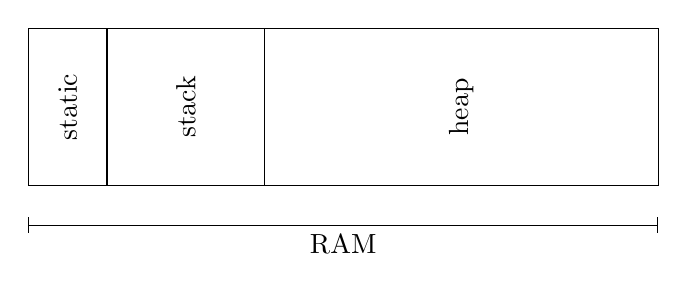
\begin{tikzpicture}
      \draw (0,0) rectangle ++(1,2);
      \draw (1,0) rectangle ++(2,2);
      \draw (3,0) rectangle ++(5,2);

      \node[rotate=90] at (0.5,1) {static};
      \node[rotate=90] at (2,1) {stack};
      \node[rotate=90] at (5.5,1) {heap};

      \draw[|-|] (0,-.5) -- ++(8,0) node[midway,below] {RAM};
    \end{tikzpicture}
  \end{center}
\end{frame}

\begin{frame}
  \frametitle{Heap Allocation}
  \notrealcpp
  \begin{columns}
    \column{5cm}
    \code[font=\small,frame=none,language=c++14]{heap-allocation.cpp}
    \column{4cm}
    \begin{center}
      \begin{tikzpicture}[allocation/.style={-latex,thick},remember picture,overlay,scale=.5]
        \coordinate (start) at (-4,4);

        \only<handout:1-|3->{
          \draw[fill=red!50] (start) rectangle ++(4,-1);
        }
        \only<handout:1|3>{
          \draw[allocation] (var a) to [bend left=30] ($ (start) + (0,-.5) $);
        }

        \only<handout:1-|4->{
          \draw[fill=green!50] ($ (start) + (4,0) $) rectangle ++(4,-1);
        }
        \only<handout:1|4>{
          \draw[allocation] (var b) to [bend left=30] ($ (start) + (4,-0.5) $);
        }

        \only<handout:1-|5->{
          \draw[fill=blue!50] ($ (start) + (0,-1) $) rectangle ++(4,-1);
        }
        \only<handout:1|5>{
          \draw[allocation] (var c) to [bend left=30] ($ (start) + (0,-1.5) $);
        }

        \only<handout:1-|6->{
          \draw[fill=yellow!50] ($ (start) + (4,-1) $) rectangle ++(4,-1);
        }
        \only<handout:1|6>{
          \draw[allocation] (var d) to [bend left=30] ($ (start) + (4,-1.5) $);
        }

        \only<handout:2|7-11>{
          \draw[fill=red!50] ($ (start) + (0,-2) $) rectangle ++(8,-1);
        }
        \only<handout:2|7>{
          \draw[allocation] (mem a) to [bend right=30] ($ (start) + (0,-2.5) $);
        }

        \only<handout:2|8-10>{
          \draw[fill=green!50] ($ (start) + (0,-3) $) rectangle ++(8,-3);
        }
        \only<handout:2|8>{
          \draw[allocation] (mem b) to [bend right=30] ($ (start) + (0,-3.5) $);
        }

        \only<handout:2|9-12>{
          \draw[fill=blue!50] ($ (start) + (0,-6) $) rectangle ++(8,-2);
        }
        \only<handout:2|9>{
          \draw[allocation] (mem c) to [bend right=30] ($ (start) + (0,-6.5) $);
        }

        \only<handout:2|10-13>{
          \draw[fill=yellow!50] ($ (start) + (0,-8) $) rectangle ++(8,-2);
        }
        \only<handout:2|10>{
          \draw[allocation] (mem d) to [bend right=30] ($ (start) + (0,-8.5) $);
        }

        \only<handout:3|11>{
          \draw[->,thick] (del b) ++(2,0) -- ++(-1,0);
        }

        \only<handout:3|12>{
          \draw[->,thick] (del a) ++(2,0) -- ++(-1,0);
        }

        \only<handout:3|13>{
          \draw[->,thick] (del c) ++(2,0) -- ++(-1,0);
        }

        \only<handout:3|14>{
          \draw[->,thick] (del d) ++(2,0) -- ++(-1,0);
        }

        \draw (start) grid ++(8,-10);
      \end{tikzpicture}
    \end{center}
  \end{columns}
  \vskip2cm
  \begin{overprint}
    \onslide<handout:1|2-6>
    \begin{center}
      \textbf{At compile time} \\ Compiler assigns memory locations to each global
    \end{center}

    \onslide<handout:2-3|7->
    \begin{center}
      \textbf{At runtime} \\ Arrays allocated on heap
    \end{center}
  \end{overprint}
\end{frame}

\begin{frame}
  \frametitle{Fragmentation}
  \code[language=c++14]{fragmentation.cpp}
  \begin{center}
    \begin{tikzpicture}[scale=.5]
      \foreach \i in {0,2,...,15} {
        \tikzmath{
          int \j;
          int \k;
          \j = int(\i + 2);
          \k = int(17 + int(\i / 2));
        }
        \only<\j-\k>{
          \draw[fill=red!50] (\i,0) rectangle ++(1,1);
        }
      }

      \foreach \i in {1,3,...,15} {
        \tikzmath{
          int \j;
          \j = int(\i + 2);
        }
        \only<\j-25>{
          \draw[fill=red!50] (\i,0) rectangle ++(1,1);
        }
      }

      \draw (0,0) grid (16,1);
    \end{tikzpicture}
  \end{center}
  \visible<25>{
    \begin{center}
      8 bytes free yet cannot allocate array larger than 1 byte
    \end{center}
  }
\end{frame}

\begin{frame}
  \frametitle{Heap Allocation}
  \begin{procontralist}
    \pro Allows allocation of arbitrarily large blocks
    \pro Deallocation possible in any order
    \pro Most general allocation method
    \con Requires some bookkeeping \\ (keeps track of linked list of free blocks)
    \con Deallocation necessary
    \con Allocation/Deallocation relatively slow
    \con Fragmentation
  \end{procontralist}
\end{frame}


%%% Local Variables:
%%% mode: latex
%%% TeX-master: "allocation-methods"
%%% End:
